\section{Pesquisas do Gartner}


\subsection{Estudos gerais}

A seguir, apresentamos alguns estudos do Gartner (líder mundial na
pesquisa de tecnologia de informação que também atua como empresa de consultoria):

\begin{itemise}

    \item Aproximadamente 19\% das organizações ao redor do mundo estão utilizando a
    computação em nuvem para produção de aplicações, enquanto outros 20\% contratam
    serviços públicos de armazenamento na nuvem. O principal modelo sendo utilizado é
    a da nuvem híbrida~\cite{gartner-public-cloud-services}.

    \item Consumidores armazenarão mais de 1/3 de seu conteúdo digital na nuvem por
    volta de 2016~\cite{gartner-one-third}.

    % Segundo estimativas do grupo americano de informática IBM, o mercado mundial de
    % computação em nuvem poderia alcançar os 200 bilhões de dólares em 2020.

\end{itemise}

Os resultados mostram que a nuvem oferece grandes oportunidades de negócios,
especialmente para serviços de armazenamento. 

Ao mesmo tempo, a indústria de serviços de nuvem é grande e conta com muitos 
provedores com estratégias agressivas para conquistar clientes. Para orientar as 
companhias na hora de selecionar seu parceiro, o Gartner elegeu os dez principais 
fornecedores de serviços de armazenamento~\cite{gartner-top-10}, levando em 
consideração a capacidade deles de atendimento aos clientes:

\begin{figure}[ht]
    \centering
    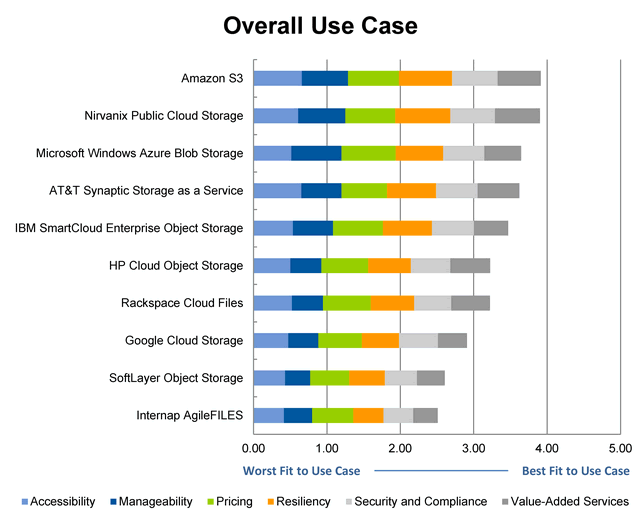
\includegraphics[width=0.8\textwidth]{img/top10.png}
    \caption{Avaliação dos dez principais fornecedores, segundo o Gartner}
\end{figure}


\subsection{Os 10 maiores mitos sobre a nuvem}

Mesmo com uma definição formal com a qual muitos concordam, várias perspectivas 
ainda contribuem para mistificar a computação em nuvem. Somado à propaganda 
incessante, a confusão resultante permeia a área de TI e além nos dias atuais. No 
final de 2014, o Gartner destacou 10 dos mitos mais perigosos e enganadores sobre a 
nuvem~\cite{gartner-10-myths-cloud}:
	
\newcommand{\itemm}[1]{\item\textbf{#1}\newline}	

\begin{enumerate}
    \itemm{A nuvem está sempre ligada ao capital}
		Apesar de os preços estarem caindo, especialmente para os IaaS, nem todos os 
		serviços de nuvem estão ficando mais baratos. Assumir que a nuvem sempre 
		traz benefícios econômicos pode levar a limitações na carreira. Economizar 
		capital pode vir a ser um dos benefícios, mas não é sempre uma certeza.

    \itemm{Você precisa estar na nuvem para ser bom}\label{item:need-to-be-cloud}
		Organizações de TI estão cada vez mais usando serviços de nuvem como parte 
		de suas tentativas de ganhar fundos e atingir demandas e estratégias da 
		nuvem. O mito resultante é que as pessoas estão caindo na armadilha de 
		acreditar que, se algo é bom, então precisa estar na nuvem.

    \itemm{A nuvem deve ser usada para tudo}
		Relacionada ao mito~\ref{item:need-to-be-cloud}, este se refere à crença de 
		que as características reais da nuvem se aplicam ou são desejáveis para 
		tudo. Claramente, há alguns casos de uso onde funcionam bem, mas nem todas 
		as aplicãções se beneficiam da nuvem. A menos que haja redução de custos, 
		mover uma aplicação legada imutável não é uma boa ideia.

    \itemm{"Mas o diretor executivo disse" é uma estratégia de nuvem}
		Quando perguntados sobre qual é sua estratégia de nuvem, muitas companhias, 
		por não terem uma, costumam dizer que só estão fazendo o que o CEO (diretor 
		executivo) quer. Isto não é uma estratégia de nuvem. Esta começa com a 
		identificação de objetivos de negócio e o mapeamento de benefícios em 
		potencial da nuvem, ao mesmo tempo em que as inconveniências são atenuadas. 
		A nuvem deve ser considerada como um meio para um determinado fim, que deve 
		ser primeiramente especificado.

    \itemm{Nós precisamos de \emph{uma} estratégia ou \emph{um} fornecedor de nuvem}
		Serviços de nuvem são vastos, com diversas camadas (IaaS, SaaS...) e 
		aplicações. Uma estratégia de nuvem deve ser baseada em alinhar os objetivos 
		de negócio com benefícios em potencial. Tais objetivos e benefícios são 
		diferentes em vários casos de uso e devem guiar as atividades comerciais, em 
		vez de servirem como tentativas de uniformizar uma oferta ou estratégia.

    \itemm{A nuvem é menos segura do que recursos instalados localmente}
		Computação em nuvem às vezes é vista como algo não tão seguro. Isso é mais 
		um problema de confiança do que baseado em uma análise razoável de 
		capacidades reais de segurança. Até pelo menos 2014 (ano de realização da 
		pesquisa), houve poucas falhas de segurança na nuvem pública --- a maioria 
		dos problemas envolve ambientes de data center locais. Apesar 
		de os fornecedores de nuvem possuírem o dever de demonstrar suas capacidades, 
		quando isso é feito não há razão para desconfiar da segurança de suas 
		ofertas.

    \itemm{A nuvem não deve ser usada para casos de risco}
		Computação em nuvem não é "tudo ou nada". Ela está sendo adotada aos poucos 
		e em casos específicos. Portanto, não é de se surpreender que casos de uso 
		iniciais geralmente não são para sistemas críticos. No entanto, muitas 
		organizações progrediram além dos casos de usos iniciais e experimentãção, e 
		estão usando a nuvem para tarefas críticas. Há também muitas empresas (não 
		apenas pequenas \emph{startups}) que "nascem na nuvem" e possuem todo o seu 
		negócio (claramente de sistemas críticos) completamente na nuvem.

    \itemm{Nuvem = Data center}
		A maioria das decisões de nuvem não são (e não deveriam ser) sobre fechar 
		completamente data centers e mover tudo para a nuvem. Uma estratégia de 
		nuvem também não deve ser equiparada a uma estratégia de data center. É 
		necessário haver espaço de data center para dados que não estão na nuvem e, 
		se forem retirados do data center, haverá consequências. Em resumo, nuvem e 
		data center não são sinônimos.

    \itemm{Migrar para a nuvem leva automaticamente ao ganho de todas as suas
                   características}
		Não se deve assumir que "migrar para a nuvem" levará automaticamente à 
		herança de todas as características da nuvem vindas de níveis mais baixos 
		(como IaaS). Os atributos da nuvem não são transitivos; deve-se distinguir 
		aplicações oferecidas na nuvem dos serviços de nuvem em si. Há alguns pontos 
		da nuvem que trazem benefícios, como não haver necessidade de comprar 
		hardware, mas tais pontos não levam aos mesmos resultados.

    \itemm{Virtualização = Nuvem privada}
		Virtualização é uma tecnologia comumente usada em computação em nuvem. No 
		entanto, não é a única maneira de se implementar uma nuvem, nem é suficiente 
		para tal implementação. Isto é relevante em discussões de nuvem privada, 
		onde ambientes altamente virtualizados e automatizados são comuns; em muitos 
		casos, é exatamente o que é necessário. Infelizmente, tais ambientes são 
		erroneamente descritos como "nuvens privadas".
\end{enumerate}
\undef\itemm
